\documentclass{article}

% Useful packages
\usepackage[letterpaper,top=2cm,bottom=2cm,left=3cm,right=3cm,marginparwidth=1.75cm]{geometry}
\usepackage{amsmath}
\usepackage{graphicx}
\usepackage[colorlinks=true, allcolors=blue]{hyperref}
\usepackage{titling}
\usepackage{float}
\usepackage[demo]{graphicx}
\usepackage[T1]{fontenc}
\usepackage[spanish]{babel}
\usepackage{tabularx}


% Useful for augmented matrix representation
\makeatletter
\renewcommand*\env@matrix[1][*\c@MaxMatrixCols c]{%
  \hskip -\arraycolsep
  \let\@ifnextchar\new@ifnextchar
  \array{#1}}
\makeatother

\usepackage{listings}
\usepackage{color}

\definecolor{dkgreen}{rgb}{0,0.6,0}
\definecolor{gray}{rgb}{0.5,0.5,0.5}
\definecolor{mauve}{rgb}{0.58,0,0.82}

\lstset{frame=tb,
  language=Matlab,
  aboveskip=3mm,
  belowskip=3mm,
  showstringspaces=false,
  columns=flexible,
  basicstyle={\small\ttfamily},
  numbers=none,
  numberstyle=\tiny\color{gray},
  keywordstyle=\color{blue},
  commentstyle=\color{dkgreen},
  stringstyle=\color{mauve},
  breaklines=true,
  breakatwhitespace=true,
  tabsize=3
}

\setcounter{section}{0}

\title{
\includegraphics[scale=0.5]{logo.jpg}\\ \textbf{Laboratorio 3} 
\\ \large APROXIMACIÓN DE FUNCIONES / INTERPOLACIÓN           
\\ \large Métodos de Computación Científica}

\author{Manuel Lagos}

\begin{document}
\setcounter{section}{-1}
\maketitle

\section{Aclaración}
Para la resolución de sistemas lineales se utilizó el software Octave, los cálculos intermedios y el código no fueron incluidos en el desarrollo para no oscurecer el mísmo. Esto es así dado que el tema resolución de sistemas lineales ya fue evaluado en el trabajo anterior.

\section{Ejercicio 1}
 Considere las siguientes aproximaciones:\\
i) $g(x) = \alpha \cdot e^{\beta x}$\\
ii) $h(x) = \alpha \cdot x^{\beta}$

a) Determine graficamente cual de estas aproximaciones parece mas adecuada para ajustar los
siguientes datos:\\
\hspace{0.5cm} $P_1 (1, 2.3) \hspace{0.5cm} P_2 (2, 6.1) \hspace{0.5cm} P_3(3, 10.7) \hspace{0.5cm} P_4 (4, 16.0) \hspace{0.5cm} P_5 (5, 21.9) \hspace{0.5cm} P_6 \hspace{0.5cm} (6, 28.3)$\\
b) Emplee el algoritmo de linealizacion para ajustar g(x) y h(x) a los datos, y ademas encuentre
$E(g) = \sum_{k=1}^m{[g(x_k)-y_k]^2}$ y $E(g) = \sum_{k=1}^m{[h(x_k)-y_k]^2}$\\
c) Confirman los resultados del inciso b su respuesta al inciso a\\ \\ \\ \\ \\ \\ \\ \\ \\ \\ \\ \\ \\ \\ \\ \\

a)

\begin{figure}[H]
    \centering
    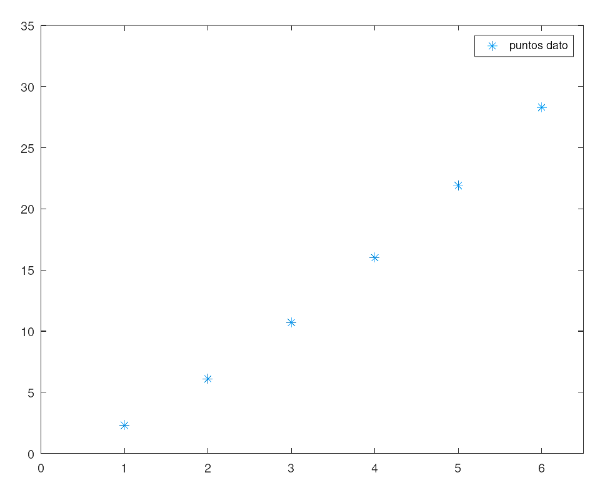
\includegraphics[width=0.7\linewidth]{ej1_datos.png}
    \label{fig:enter-label}
    \caption{A simple vista parece más adecuada la aproximación $h(x) = \alpha \cdot x^{\beta}$}
\end{figure}

b)\\

\[
g(x) = \alpha \cdot e^{\beta x}
\]
\[
ln(g(x)) = ln(\alpha) + \beta \cdot x
\]\\

por cuadrados mínimos, si $y = a + b \cdot x$ con m datos entonces:
\vspace{0.5cm}
\[
\begin{bmatrix}
    m & \sum{x_k} \\
    \sum{x_k} & \sum{x_k^2}
\end{bmatrix}
\cdot
\begin{bmatrix}
    a \\ b
\end{bmatrix}
=
\begin{bmatrix}
    \sum{y_k} \\
    \sum{x_k \cdot y_k}
\end{bmatrix}
\]

en este caso: $y = ln(g(x))$, $ln(\alpha) = a$, $\beta = b$, y según los datos:
\begin{table}[H]
\centering
\begin{tabular}{|l|l|l|l|l|l|}
\hline
  & $x$  & $y$ & $x^2$ & $ln(g(x))$  & $x \cdot ln(g(x))$ \\ \hline
  & 1  & 2.3  & 1                    & 0.833  & 0.833   \\
  & 2  & 6.1  & 4                    & 1.808  & 3.617   \\
  & 3  & 10.7 & 9                    & 2.370  & 7.111   \\
  & 4  & 16.0 & 16                   & 2.773  & 11.090  \\
  & 5  & 21.9 & 25                   & 3.086  & 15.432  \\
  & 6  & 28.3 & 36                   & 3.343  & 20.057  \\ \hline
$\sum$ & 21 & 85.3 & 91                   & 14.213 & 58.14   \\ \hline
\end{tabular}
\end{table}

luego,

\[
\begin{bmatrix}
    6 & 21 \\
    21 & 91
\end{bmatrix}
\cdot
\begin{bmatrix}
    a \\ b
\end{bmatrix}
=
\begin{bmatrix}
    14.213 \\
    58.14
\end{bmatrix}
\]\\

resolviendo el sistema:

\[a = 0.690\]
\[b = 0.4796\]

tenemos que,

\[ln(\alpha) = a\]
\[\alpha = e^a\]
\[\alpha = 1.994\],

luego,

\[g(x)=1.994 \cdot e^{0.4796 \cdot x}\]\\

la suma del cuadrado de los residuos es:

\[
E(g) = \sum_{k=1}^{6}{[g(x_k)-y_k]^2} = 63.646
\]\\

\[
h(x) = \alpha \cdot x^{\beta}
\]
\[
ln(h(x)) = ln(\alpha) + \beta \cdot ln(x)
\]\\

por cuadrados mínimos, si $y = a + b \cdot x$ con m datos entonces:
\vspace{0.5cm}
\[
\begin{bmatrix}
    m & \sum{x_k} \\
    \sum{x_k} & \sum{x_k^2}
\end{bmatrix}
\cdot
\begin{bmatrix}
    a \\ b
\end{bmatrix}
=
\begin{bmatrix}
    \sum{y_k} \\
    \sum{x_k \cdot y_k}
\end{bmatrix}
\]

en este caso: $y = ln(h(x))$, $ln(\alpha) = a$, $\beta = b$, $x=ln(x)$ y según los datos:
\begin{table}[H]
\centering
\begin{tabular}{|l|l|l|l|l|l|l|}
\hline
  & $x$  & $y$    & $ln(x)$ & $ln(y)$  & $ln(x)^2$ & $ln(x) \cdot ln(y)$ \\ \hline
  & 1  & 2.3  & 0     & 0.833  & 0                        & 0           \\
  & 2  & 6.1  & 0.693 & 1.808  & 0.48                     & 1.253       \\
  & 3  & 10.7 & 1.099 & 2.370  & 1.207                    & 2.604       \\
  & 4  & 16.0 & 1.386 & 2.773  & 1.922                    & 3.844       \\
  & 5  & 21.9 & 1.609 & 3.086  & 2.59                     & 4.968       \\
  & 6  & 28.3 & 1.792 & 3.343  & 3.21                     & 5.99        \\ \hline
s & 21 & 85.3 & 6.579 & 14.213 & 9.409                    & 18.659      \\ \hline
\end{tabular}
\end{table}

luego,

\[
\begin{bmatrix}
    6 & 6.579 \\
    6.579 & 9.409
\end{bmatrix}
\cdot
\begin{bmatrix}
    a \\ b
\end{bmatrix}
=
\begin{bmatrix}
    14.213 \\
    18.659
\end{bmatrix}
\]

resolviendo el sistema:

\[a = 0.834\]
\[b = 1.34\]

tenemos que,

\[ln(\alpha) = a\]
\[\alpha = e^a\]
\[\alpha = 2.303\]

luego,

\[h(x)=2.303 \cdot x^{1.34}\]

la suma del cuadrado de los residuos es:

\[
E(h) = \sum_{k=1}^{6}{[h(x_k)-y_k]^2} = 2.5469 \cdot 10^{-3}
\]\\

c)

\begin{figure}[H]
    \centering
    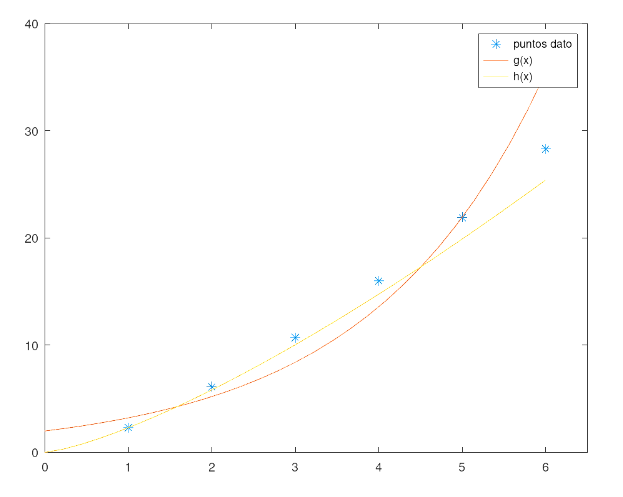
\includegraphics[width=1\linewidth]{ej1_a.png}
    \label{fig:enter-label}
    \caption{comparación entre los datos, g(x) y h(x)}
\end{figure}

\[ 
E(g) > E(h)
\]
\[
63.793  > 2.5469 \cdot 10^{-3}
\]

Efectivamente, la aproximación h ajusta mejor a los datos como se supuso en el primer inciso.

\section{Ejercicio 2}
De acuerdo a la Figura 1, los polinomios interpoladores para la función $\dfrac{1}{(1 + x^2)}$ en el
intervalo $[−3, 3]$ basados en puntos igualmente espaciados son muy inexactos cerca de los extremos
del intervalo.\\
2.1 Realice interpolaciones por spline cúbica natural basadas en los mismos 3, 5 y 11 puntos dato.\\
2.2 Compare con la Figura 3 los gráficos obtenidos en la sección 2.1. Exhibe la técnica de
interpolación por spline la misma inexactitud?.\\

\begin{figure}[H]
    \centering
    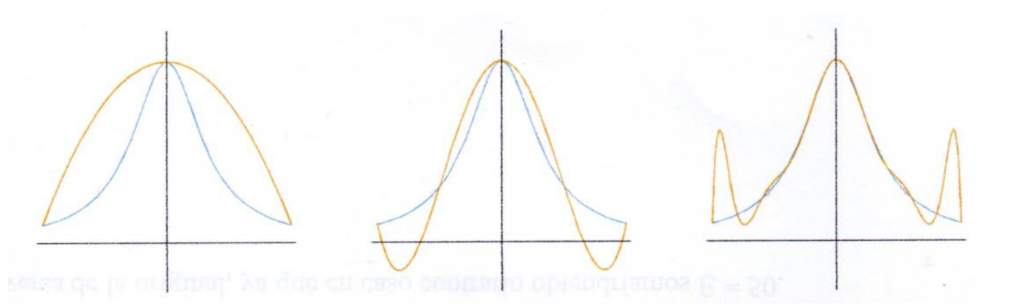
\includegraphics[width=1\linewidth]{Screenshot_20231019_181840.png}
    \label{fig:enter-label}
    \caption{Polinomios de interpolación de grados 2, 4 y 10 para la función  $\dfrac{1}{(1 + x^2)}$}
\end{figure}

2.1\\
Interpolación por spline cúbica natural basada en tres puntos datos igualmente espaciados, en el intervalo $[-3, 3]$.\\

\begin{table}[H]
\centering
\begin{tabular}{|l|l|l|}
\hline
$i$ & $t_i$ & $y_i$ \\ \hline
0 & -3   & $1/10$ \\ \hline
1 & 0    & 1    \\ \hline
2 & 3    & 1/10 \\ \hline
\end{tabular}
\end{table}

buscamos 

\[ S(x) = \begin{cases} 
      S_o(x) & x \in [-3, 0] \\
      S_1(x) & x \in [0, 3]
   \end{cases}
\]\\

con $S_i(x) = a_i \cdot x^3 + b_i \cdot x^2 + c_i \cdot x + d_i$, $i = 0, 1$.
dado que tenemos cuatro incógnitas por ecuación y dos ecuaciones, tenemos ocho incógnitas, por lo que se necesitan ocho ecuaciones.\\

Según las condiciones de interpolación:
\begin{itemize}
    \item para el punto interior:\\$S_{i-1}(t_i) = y_i = S_i(t_i)$\\
    luego, 
    \[S_0(0) = a_0 \cdot 0^3 + b_0 \cdot 0^2 + c_0 \cdot 0 + d_0 = 1\]
    y, 
    \[S_1(0) = a_1 \cdot 0^3 + b_1 \cdot 0^2 + c_1 \cdot 0 + d_1 = 1\]

    por lo que $d_0 = d_1 = 1$
    
    \item para los extremos:\\
    $S_0(t_0) = y_o$\\
    luego,
    \[S_0(-3) = -27 \cdot a_0 + 9 \cdot b_0 -3 \cdot c_0 + d_0 = \dfrac{1}{10} \]
    y,
    \[S_1(-3) = 27 \cdot a_1 + 9 \cdot b_1 3 \cdot c_1 + d_1 = \dfrac{1}{10} \]
\end{itemize}

Según las condiciones de continuidad:
\begin{itemize}
    \item $S^{'}_{i-1}(t_i)=S^{'}_{i}(t_i)$\\
    \[S^{'}_{0}(0)=S^{'}_{1}(0)\]
    \[3 \cdot a_0 \cdot 0^2 + 2 \cdot b_0 \cdot 0 + c_0 = 3 \cdot a_1 \cdot 0^2 + 2 \cdot b_1 \cdot 0 + c_1\]
    \[0 \cdot a_0 + 0 \cdot b_0 + c_0 = 0 \cdot a_1 + 0 \cdot b_1 + c_1\]
    \[0 \cdot a_0 + 0 \cdot b_0 + c_0 - 0 \cdot a_1 - 0 \cdot b_1 - c_1 = 0\]
    por lo que $c_0 = c_1$

    \item $S^{''}_{i-1}(t_i)=S^{''}_{i}(t_i)$\\
    \[S^{''}_{0}(0)=S^{''}_{1}(0)\]
    \[6 \cdot a_0 \cdot 0 + 2 \cdot b_0 = 6 \cdot a_1 \cdot 0 + 2 \cdot b_0 \]
    \[0 \cdot a_0 + 2 \cdot b_0 = 0 \cdot a_1 + 2 \cdot b_1 \]
    \[0 \cdot a_0 + 2 \cdot b_0 - 0 \cdot a_1 - 2 \cdot b_1 = 0\]
    por lo que $b_0 = b_1$
\end{itemize}

Según las condiciones de extremo (Spline Cúbica Natural):
\begin{itemize}
    \item $S^{''}_0(t_0)=0$\\
    \[6 \cdot a_0 \cdot -3 + 2 \cdot b_0 = 0\]
    \item $S^{''}_1(t_2)=0$\\
    \[6 \cdot a_1 \cdot 3 + 2 \cdot b_1 = 0\]
    dado que $b_0 = b_1$ luego $a_0=-a_1$
\end{itemize}\\

Expresando las ocho ecuaciones en forma matricial:\\

\[
A \cdot x = b \implies
\begin{bmatrix}
    0 & 0 & 0 & 1 & 0 & 0 & 0 & 0 \\
    0 & 0 & 0 & 0 & 0 & 0 & 0 & 1 \\
    -27 & 9 & -3 & 1 & 0 & 0 & 0 & 0 \\
    0 & 0 & 0 & 0 & 27 & 9 & 3 & 1 \\
    0 & 0 & 1 & 0 & 0 & 0 & -1 & 0 \\
    0 & 2 & 0 & 0 & 0 & -2 & 0 & 0 \\
    -18 & 2 & 0 & 0 & 0 & 0 & 0 & 0 \\
    0 & 0 & 0 & 0 & 18 & 2 & 0 & 0 \\
\end{bmatrix} 
\cdot
\begin{bmatrix}
    a_0 \\ b_0 \\ c_0 \\ d_0 \\ a_1 \\ b_1 \\ c_1 \\ d_1 
\end{bmatrix}
=
\begin{bmatrix}
    0 \\ 0 \\ 0.1 \\ 0.1 \\ 0 \\ 0 \\ 0 \\ 0
\end{bmatrix}
\]

La solución del sistema utilizando Octave es:

\[x = 
\begin{bmatrix}
-0.0167 & -0.15 & 0 & 1 & 0.0167 & -0.15 & 0 & 1 
\end{bmatrix}^T\]

luego,
\[ S(x) = \begin{cases} 
      S_0(x) = -0.0167 \cdot x^3 -0.15 \cdot x^2 + 1 & x \in [-3, 0] \\
      S_1(x) = 0.0167 \cdot x^3 -0.15 \cdot x^2 + 1 & x \in [0, 3]
   \end{cases}
\]\\

\begin{figure}[H]
    \centering
    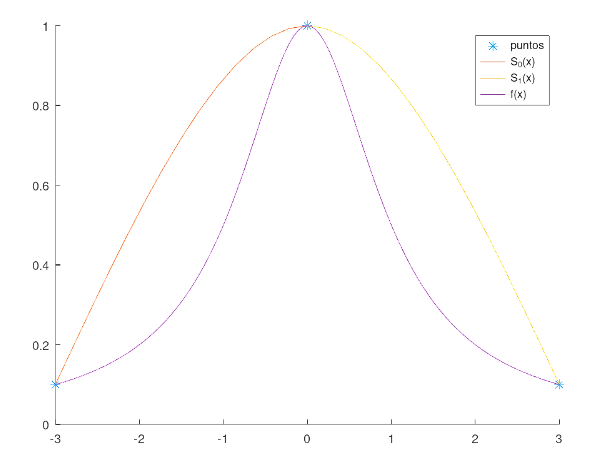
\includegraphics[width=0.5\linewidth]{Screenshot_20231020_150719.png}
    \label{fig:enter-label}
    \caption{Interpolación por spline cúbica natural basada en tres puntos datos igualmente espaciados}
\end{figure}

\textbf{Para la interpolación por spline con cinco y once puntos se usó la función provista por Octave:}
\begin{figure}[H]
    \centering
    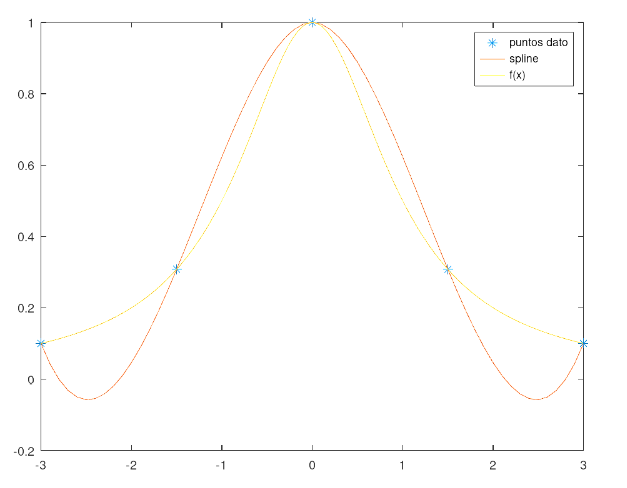
\includegraphics[width=0.5\linewidth]{spline.5.png}
    \label{fig:enter-label}
    \caption{Interpolación por spline cúbica natural basada en cinco puntos datos igualmente espaciados}
\end{figure}
\begin{figure}[H]
    \centering
    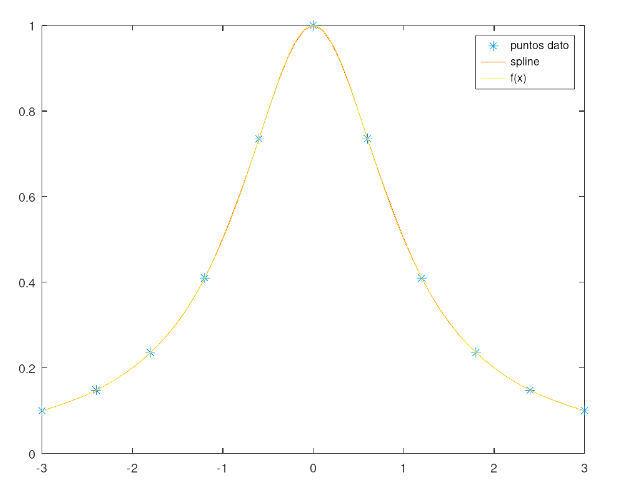
\includegraphics[width=0.5\linewidth]{spline.11.png}
    \label{fig:enter-label}
    \caption{Interpolación por spline cúbica natural basada en once puntos datos igualmente espaciados}
\end{figure}

Código:

\begin{lstlisting}
n = 11;    % cantidad de puntos dato
ini = -3;  % valor inicial
fin = 3;   % valor final
y = @(x) 1./(1+(x.^2)); % defini la función

x = linspace(ini, fin, n); % generar n puntos datos
y = y(x);                  % evaluar la función en los puntos dato

xx = ini:.1:fin;           % puntos donde evaluar la spline
yy = spline(x,y,xx);       % calcular la spline

% mostrar el resultado de la spline
plot(x,y,'*',xx,yy);

% graficar f(x)
hold on;
fplot("1/(1+x^2)", [ini fin]);

% mostrar referencias
legend("puntos dato", "spline", "f(x)");

\end{lstlisting}

\\
2.2
Comparando la figura 3 con los resultados obtenidos se observa claramente una mayor exactitud con la ténica de interpolación por splines cúbicas. Esto es así ya que con muchos puntos, el método de Lagrange para polinomios de grado relativamente alto sufre de oscilaciones anormales, especialmente cerca de los extremos del intervalo, esto se connoce como efecto Runge. Mientras que el método por Splines no lo padece, debido a que, al partir la función en intervalos, cada $S_i(x)$ es un polinomio de grado relativamente bajo. Una solución alternativa podría ser realizar un ajuste mixto, o en lugar de usar nodos equidistantes usar nodos de Chebyshov. \\
\vspace{3cm}
\section{Ejercicio 3}
Chen y Saxena reportaron los siguientes datos experimentales para la emisividad e del
tungsteno en función de la temperatura T:\\
\begin{figure}[H]
    \centering
    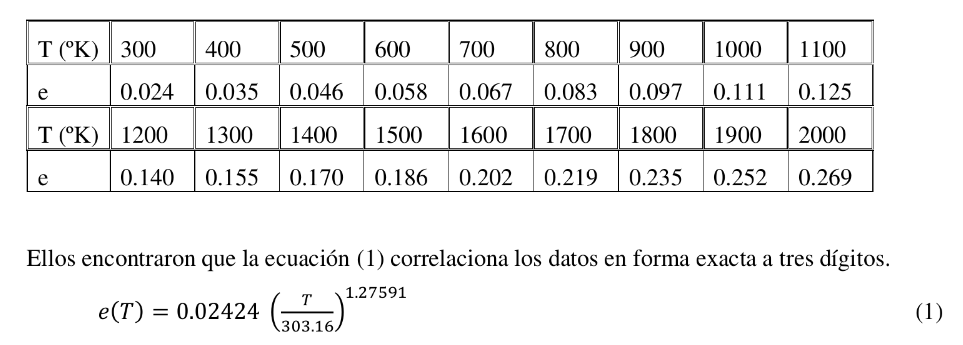
\includegraphics[width=1\linewidth]{ej3.png}
    \label{fig:enter-label}
\end{figure}\\

a) Qué grado se requiere del polinomio interpolador tal que sus aproximaciones se correspondan con
la correlación (1) en los puntos que están localizados a medio camino entre las temperaturas
tabuladas? \\
b) Discuta los pros y contras de la interpolación polinomial en comparación con usar su correlación.\\

a) Si se realiza una interpolación por el método de Lagrange con los diecinueve puntos de la tabla, se necesita un polinomio de a lo sumo grado dieciocho. Esto es así debido a que con la interpolación se busca que la función interpoladora coincida exactamente con cada uno de los puntos dato. Si además se agregan los dieciseis puntos intermedios utilizando la correlación (1) como e valor de referencia, con treinta y cinco puntos se necesita un polinomio de a lo sumo grado treinta y cuatro. Claramente esto es poco práctico, además que sufriría del efecto Runge en gran manera. Es más razonable utilizar tan solo algunos puntos de la tabla elegidos inteligentemente y bien distribuidos. A continuación se muestran algunos experimentos.

\begin{figure}[H]
    \centering
    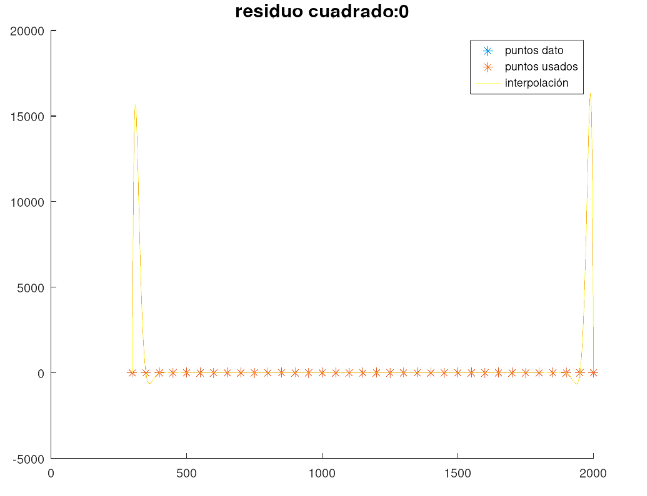
\includegraphics[width=0.7\linewidth]{35.png}
    \label{fig:enter-label}
    \caption{interpolación por el método de Lagrande utilizando los diecinueve puntos de la tabla más los puntos intermedios calculados con la correlación $e(T)$, para observar el fenómeno de Runge}
\end{figure}\\

\begin{figure}[H]
    \centering
    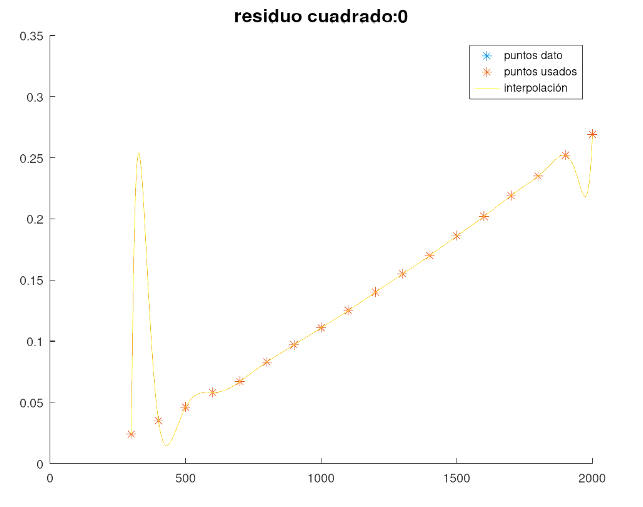
\includegraphics[width=0.7\linewidth]{19.png}
    \label{fig:enter-label}
    \caption{interpolación por el método de Lagrande utilizando los diecinueve puntos de la tabla, para observar el fenómeno de Runge}
\end{figure}\\

\begin{figure}[H]
    \centering
    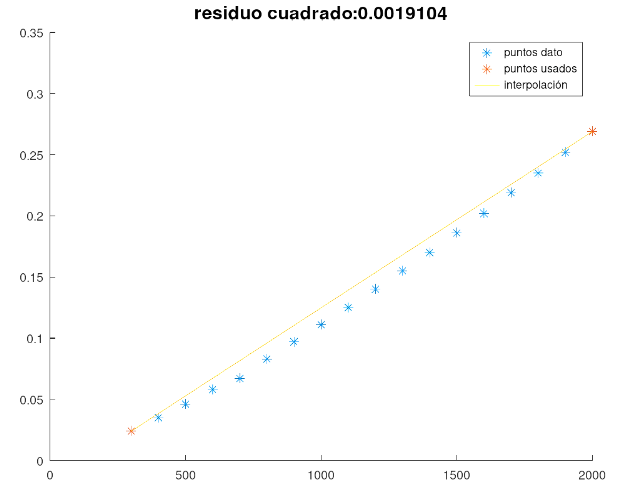
\includegraphics[width=0.7\linewidth]{2.png}
    \label{fig:enter-label}
    \caption{interpolación por el método de Lagrande utilizando los dos puntos de los extremos}
\end{figure}\\

\begin{figure}[H]
    \centering
    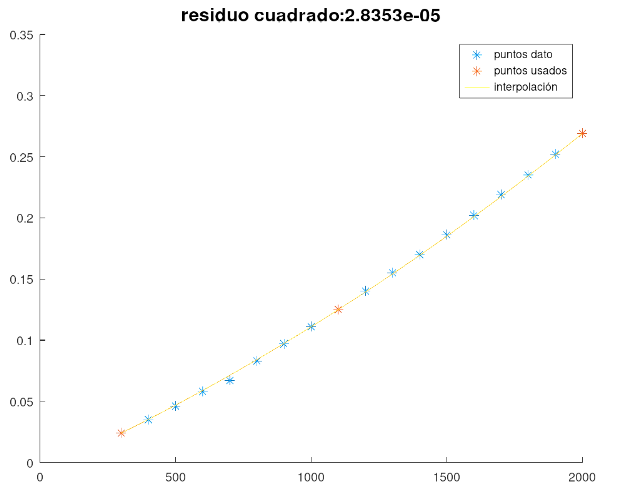
\includegraphics[width=0.7\linewidth]{3.png}
    \label{fig:enter-label}
    \caption{interpolación por el método de Lagrande utilizando tres puntos relativamente igualmente espaciados}
\end{figure}\\

\begin{figure}[H]
    \centering
    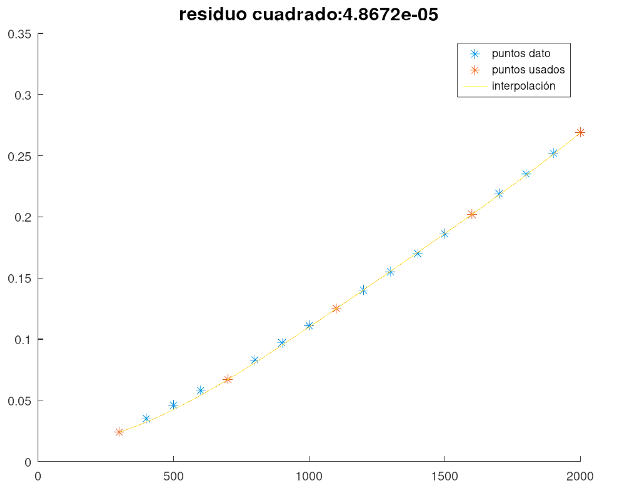
\includegraphics[width=0.7\linewidth]{5.png}
    \label{fig:enter-label}
    \caption{interpolación por el método de Lagrande utilizando cinco puntos relativamente igualmente espaciados}
\end{figure}\\

b)
La ventaja de la interpolación polinomial es que el residuo en los puntos utilizados es exactamente cero. Sin embargo, esto se logra utilizando un polinomio de grado a lo sumo la cantidad de puntos utilizados (menos uno), por lo que si se tienen relativamente muchos puntos el polinomio resulta considerablemente grande además de ser más complejo de computar. Pero la principal desventaja es que al agregar un nuevo punto dato, se debe volver a calcular todo el polinomio de cero, para adaptar el modelo a la nueva medición. En conclusión el método es principalmente útil cuando se tienen pocos y confiables datos, y se sabe que no se agregaran o quitarán otros. Si la cantidad de puntos dato es fija, es posible evitar el fenómeno de Runge con el método por Slines. En cualquier otro caso es preferible realizar una aproximación por cuadrados mínimos. \\

código:
\begin{lstlisting}
clf; % limpiar el gráfico
clc; % limpiar la consola

% t es un valor donde evaluar la función
% x son las absisas de los puntos dato
% y son las ordenadas de los puntos dato
function res = lagrange(t, x, y)
  if (size(x) != size(y))
    printf("ERROR: las dim. de x e y deben coincidir\n");
  end

  n = size(x)(2);
  h = abs(x(1)-x(2));
  suma = 0;

  for i = 0:n-1
    prod1 = 1; prod2 = 1;
    for k = 0:n-1
      if (k != i)
        prod1 *= t - x(k+1);
        prod2 *= x(i+1) - x(k+1);
      end
    end

    suma += (prod1/prod2) * y(i+1);
  end

  res = suma;
end

% función de correlación que aproxima a los datos
%aprox = @(T) 0.02424 * (T/303.16)^(1.27591);

% calcula el residuo cuadrado
function err = obtenerResiduoCuadrado(x, y, f)

  if (size(x) != size(y))
    printf("ERROR: las dim. de x e y no coinciden o n no es un num nat.\n");
    return;
  end

  err = 0;

  for i=0:size(x)(2)-1
    err += (f(x(i+1))-y(i+1))^2
  end
end

% puntos dato
x_0 = [300, 400, 500, 600, 700, 800, 900, 1000, 1100, 1200, 1300, 1400, 1500, 1600, 1700, 1800, 1900, 2000];
y_0 = [0.024, 0.035, 0.046, 0.058, 0.067, 0.083, 0.097, 0.111, 0.125, 0.140, 0.155, 0.170, 0.186, 0.202, 0.219, 0.235, 0.252, 0.269];

%x_0 = [300, 350, 400, 450, 500, 550, 600, 650, 700, 750, 800, 850, 900, 950, 1000, 1050, 1100, 1150, 1200, 1250, 1300, 1350, 1400, 1450, 1500, 1550, 1600, 1650, 1700, 1750, 1800, 1850, 1900, 1950, 2000];
%y_0 = [0.024, aprox(350), 0.035, aprox(450), 0.046, aprox(550), 0.058, aprox(650), 0.067, aprox(750), 0.083, aprox(850), 0.097, aprox(950), 0.111, aprox(1050), 0.125, aprox(1150), 0.140, aprox(1250), 0.155, aprox(1350), 0.170, aprox(1450), 0.186, aprox(1550), 0.202, aprox(1650), 0.219, aprox(1750), 0.235, aprox(1850), 0.252, aprox(1950), 0.269];

% graficar puntos dato
hold on;
plot(x_0, y_0, '*');

% puntos utilizados
x = [300, 1100, 2000];
y = [0.024, 0.125, 0.269];

% graficar puntos usados
hold on;
plot(x, y, '*');

% graficar la interpolación
x_eval = linspace(300, 2000, 1000);
y_eval = zeros(size(x_eval));

for i = 1:length(x_eval)
    y_eval(i) = lagrange(x_eval(i), x, y);
end

plot(x_eval, y_eval);

% calcular residuo cuadrado
err = obtenerResiduoCuadrado(x_0, y_0, @(t) lagrange(t, x, y))

% establecer las referencias
legend("puntos dato", "puntos usados", "interpolación");
title(strcat("residuo cuadrado: ", num2str(err)), 'FontSize', 15);
\end{lstlisting}

\section{Ejercicio 4}
Para $n = 0, 1, 2, \dots, 5$, ajuste un polinomio de grado n mediante \textbf{Cuadrados Mínimos} empleando los siguientes datos: 

\begin{figure}[H]
    \centering
    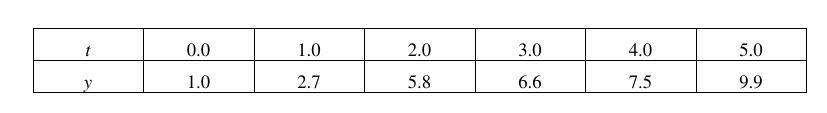
\includegraphics[width=1\linewidth]{ej4_c.png}
    \label{fig:enter-label}
\end{figure}

a) Grafique los puntos dato originales junto con cada curva polinomial resultante (puede hacer
gráficos separados para cada curva, ó un único gráfico que contenga todas las curvas)\\
b) ¿Cuál polinomio captura mejor la tendencia general de los datos? Justifique su respuesta.
Nota: Obviamente esta pregunta es subjetiva y su respuesta depende de dos factores relevantes:
la naturaleza de los datos (por ejemplo, la incertidumbre de los valores dato) y el propósito con
que se realiza el ajuste.\\

Para $n=0$\\\\
Por cuadrados mínimos, con m datos y si 
$g_0(t)=a$ 
\[
\begin{bmatrix}
    m
\end{bmatrix}
\cdot
\begin{bmatrix}
    a
\end{bmatrix}
=
\begin{bmatrix}
    \sum{y_k}
\end{bmatrix}
\]
\[
\begin{bmatrix}
    6
\end{bmatrix}
\cdot
\begin{bmatrix}
    a
\end{bmatrix}
=
\begin{bmatrix}
    33.5
\end{bmatrix}
\]
\[a = 5.583\]
luego,
\[g_0(t)=5.583\]

\begin{figure}[H]
    \centering
    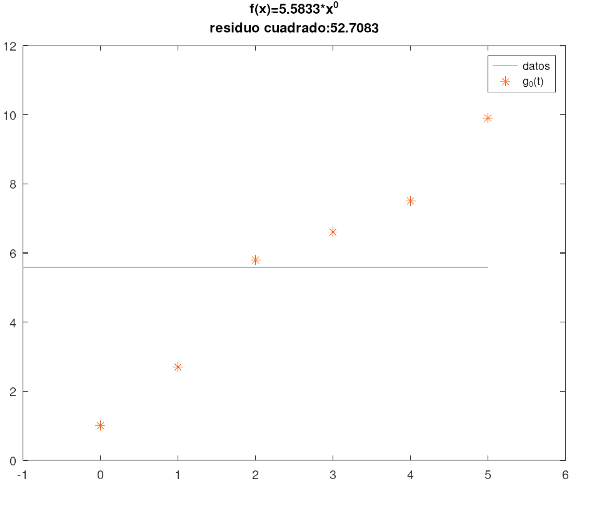
\includegraphics[width=0.6\linewidth]{grado.0.png}
    \label{fig:enter-label}
    \caption{datos vs. ajuste g_0(t)}
\end{figure}

Para $n=1$\\\\
Por cuadrados mínimos, con m datos y si 
$g_1(t)=a+ b \cdot t$
\[
\begin{bmatrix}
    m & \sum{t_k} \\
    \sum{t_k} & \sum{t_k^2}
\end{bmatrix}
\cdot
\begin{bmatrix}
    a \\ b
\end{bmatrix}
=
\begin{bmatrix}
    \sum{y_k} \\
    \sum{t_k \cdot y_k}
\end{bmatrix}
\]\\

según los datos:

\begin{table}[H]
\centering
\begin{tabular}{|l|l|l|l|l|}
\hline
  & $t$  & $y$    & $t^2$ & $t \cdot y$   \\ \hline
  & 0  & 1    & 0  & 0     \\
  & 1  & 2.7  & 1  & 2.7   \\
  & 2  & 5.8  & 4  & 11.6  \\
  & 3  & 6.6  & 9  & 19.8  \\
  & 4  & 7.5  & 16 & 30    \\
  & 5  & 9.9  & 25 & 49.5  \\ \hline
$\sum $ & 15 & 33.5 & 55 & 113.6 \\ \hline
\end{tabular}
\end{table}

\[
\begin{bmatrix}
    6 & 15 \\
    15 & 55
\end{bmatrix}
\cdot
\begin{bmatrix}
    a \\ b
\end{bmatrix}
=
\begin{bmatrix}
    33.5 \\
    113.6
\end{bmatrix}
\]

resolviendo el sistema:

\[
a = 1.319
\]
\[
b = 1.706
\]

luego,

\[g_1(t)= 1.319 + 1.706 \cdot t\]

\begin{figure}[H]
    \centering
    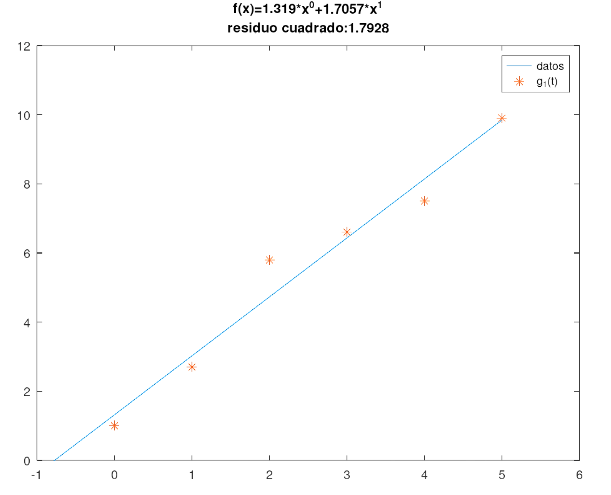
\includegraphics[width=0.6\linewidth]{grado.1.png}
    \label{fig:enter-label}
    \caption{datos vs. ajuste g_1(t)}
\end{figure}

Para $n=2$\\\\
Por cuadrados mínimos, con m datos y si 
$g_2(t)=a + b \cdot t + c \cdot t^2$
\[
\begin{bmatrix}
    m & \sum{t_k} & \sum{t_k^2} \\
    \sum{t_k} & \sum{t_k^2} & \sum{t_k^3}\\
    \sum{t_k^2} & \sum{t_k^3} & \sum{t_k^4}
\end{bmatrix}
\cdot
\begin{bmatrix}
    a \\ b \\ c
\end{bmatrix}
=
\begin{bmatrix}
    \sum{y_k} \\
    \sum{t_k \cdot y_k}\\
     \sum{t_k^2 \cdot y_k}
\end{bmatrix}
\]

según los datos:

\begin{table}[H]
\centering
\begin{tabular}{|l|l|l|l|l|l|l|l|}
\hline
  & $t$  & $y$ & $t^2$ & $t^3$  & $t^4$   & $t \cdot y$   & $t2 \cdot y$  \\ \hline
  & 0  & 1    & 0  & 0   & 0    & 0     & 0     \\
  & 1  & 2.7  & 1  & 1   & 1    & 2.7   & 2.7   \\
  & 2  & 5.8  & 4  & 8   & 16   & 11.6  & 23.2  \\
  & 3  & 6.6  & 9  & 27  & 81   & 19.8  & 59.4  \\
  & 4  & 7.5  & 16 & 64  & 256  & 30    & 120   \\
  & 5  & 9.9  & 25 & 125 & 625  & 49.5  & 247.5 \\ \hline
$\sum$ & 15 & 33.5 & 55 & 225 & 979 & 113.6 & 452.8 \\ \hline
\end{tabular}
\end{table}

\[
\begin{bmatrix}
    6 & 15 & 55 \\
    15 & 55 & 225 \\
    55 & 225 & 979
\end{bmatrix}
\cdot
\begin{bmatrix}
    a \\ b \\ c
\end{bmatrix}
=
\begin{bmatrix}
    33.5 \\
    113.6\\
    452.8
\end{bmatrix}
\]

resolviendo el sistema:

\[
a = 1.004
\]
\[
b = 2.179
\]
\[
c = -0.095
\]

luego,

\[g_2(t)=1.004 + 2.179 \cdot t -0.095 \cdot t^2\]

\begin{figure}[H]
    \centering
    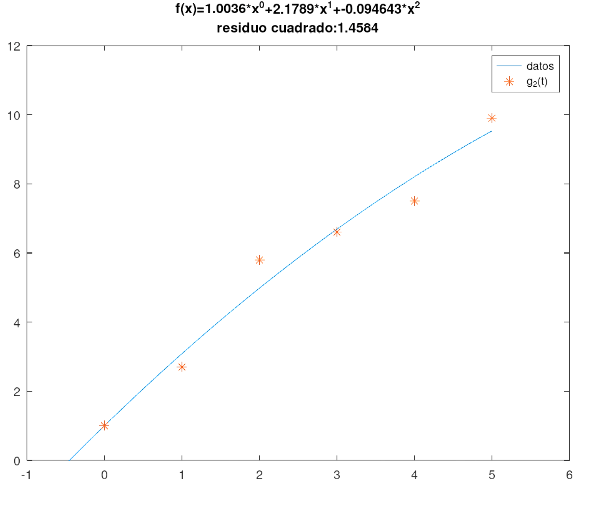
\includegraphics[width=0.6\linewidth]{grado.2.png}
    \label{fig:enter-label}
    \caption{datos vs. ajuste g_2(t)}
\end{figure}

Para los siguientes valores de n, se desarrolló un programa en Octave. Al final del ejercicio se muestra el código.\\

para n = 3\\

Por cuadrados mínimos, con m datos y si 
$g_3(t)=a + b \cdot t + c \cdot t^2 + d \cdot t^3$\\

\[
\begin{bmatrix}
    6 & 15 & 55 & 255\\
    15 & 55 & 225 & 979 \\
    55 & 225 & 979 & 4425\\
    255 & 979 & 4425 & 20515
\end{bmatrix}
\cdot
\begin{bmatrix}
    a \\ b \\ c \\ d
\end{bmatrix}
=
\begin{bmatrix}
    33.5 \\
    113.6 \\
    452.8 \\
    1944.8
\end{bmatrix}
\]

\[
\begin{bmatrix}
    a \\ b \\ c \\ d
\end{bmatrix}
=
\begin{bmatrix}
    0.789683 \\
    3.155688 \\
    -0.629365\\
    0.071296 \\
\end{bmatrix}
\]

luego,
\[g_3(t)=0.789683 + 3.155688 \cdot t -0.629365 \cdot t^2 + 0.071296 \cdot t^3\]

\begin{figure}[H]
    \centering
    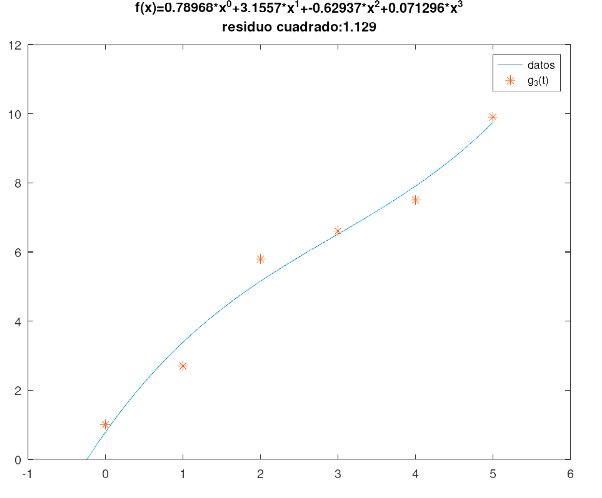
\includegraphics[width=0.6\linewidth]{grado.3.png}
    \label{fig:enter-label}
    \caption{datos vs. ajuste g_3(t)}
\end{figure}

para n = 4\\

Por cuadrados mínimos, con m datos y si 
$g_4(t)=a + b \cdot t + c \cdot t^2 + d \cdot t^3 + e \cdot t^4$\\

\[
\begin{bmatrix}
    6 & 15 & 55 & 255 & 979\\
    15 & 55 & 225 & 979 & 4425\\
    55 & 225 & 979 & 4425 & 20515\\
    255 & 979 & 4425 & 20515 & 96825\\
    979 & 4425 & 20515 & 96825 & 462979
\end{bmatrix}
\cdot
\begin{bmatrix}
    a \\ b \\ c \\ d \\ e
\end{bmatrix}
=
\begin{bmatrix}
    33.5 \\
    113.6 \\
    452.8 \\
    1944.8 \\
    8737.6
\end{bmatrix}
\]

\[
\begin{bmatrix}
    a \\ b \\ c \\ d \\ e
\end{bmatrix}
=
\begin{bmatrix}
   0.9718 \\
   0.1200 \\
   2.6340 \\
  -0.9912 \\
   0.1063 \\
\end{bmatrix}
\]

luego,
\[g_4(t)=0.97183+0.11997 \cdot x^1+2.634 \cdot x^2-0.9912 \cdot x^3+0.10625 \cdot x^4\]

\begin{figure}[H]
    \centering
    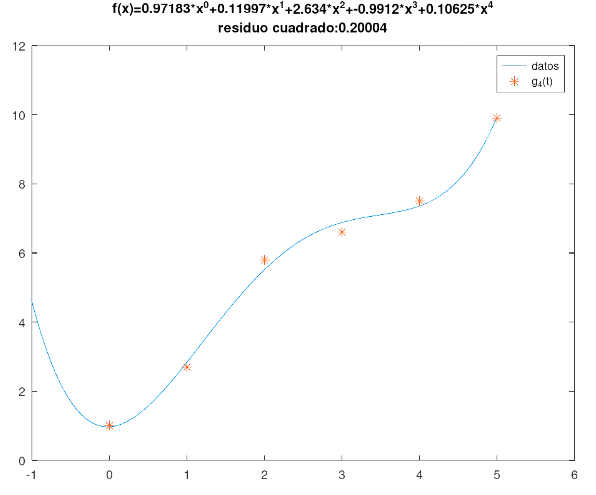
\includegraphics[width=0.6\linewidth]{grado.4.png}
    \label{fig:enter-label}
    \caption{datos vs. ajuste g_4(t)}
\end{figure}

para n = 5\\

Por cuadrados mínimos, con m datos y si 
$g_5(t)=a + b \cdot t + c \cdot t^2 + d \cdot t^3 + e \cdot t^4 + f \cdot t^5$\\

\[
\begin{bmatrix}
    6 & 15 & 55 & 255 & 979 & 4425\\
    15 & 55 & 225 & 979 & 4425 & 20515\\
    55 & 225 & 979 & 4425 & 20515 & 96825 \\
    255 & 979 & 4425 & 20515 & 96825 & 462979 \\
    979 & 4425 & 20515 & 96825 & 462979 & 2235500 \\
    4425 & 20515 & 96825 & 462979 & 2235500 & 10874000 
\end{bmatrix}
\cdot
\begin{bmatrix}
    a \\ b \\ c \\ d \\ e \\ f
\end{bmatrix}
=
\begin{bmatrix}
    33.5 \\
    113.6 \\
    452.8 \\
    1944.8 \\
    8737.6 \\
    4041
\end{bmatrix}
\]

\[
\begin{bmatrix}
    a \\ b \\ c \\ d \\ e \\ f
\end{bmatrix}
=
\begin{bmatrix}
   1 \\
  -3.178333 \\
   8.304167 \\
  -4.212500 \\
   0.845833 \\
  -0.059167 \\
\end{bmatrix}
\]

luego,
\[g_5(t)=1-3.1783 \cdot x^1+8.3042 \cdot x^2 -4.2125 \cdot x^3+0.84583 \cdot x^4 -0.059167 \cdot x^5\]

\begin{figure}[H]
    \centering
    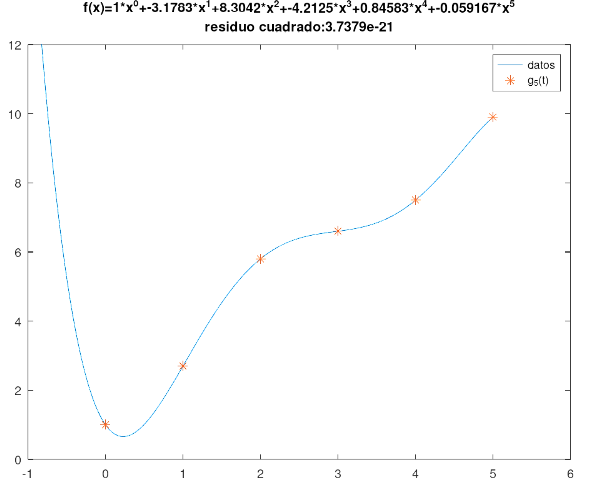
\includegraphics[width=0.6\linewidth]{grado.5.png}
    \label{fig:enter-label}
    \caption{datos vs. ajuste g_5(t)}
\end{figure}

Código del programa:

\begin{lstlisting}
x = 0; % inicializar x
y = 0; % inicializar y

function coeficientes = polinomio_cm(n, x, y)
  if (size(x) != size(y) || n < 0)
    printf("ERROR: las dim. de x e y no coinciden o n no es un num nat.\n");
    return;
  end

  m = size(x)(2);  % cantidad de datos
  A = zeros(n, n); % matriz A
  b = zeros(1, n); % vector b
  Q = {n};         % arreglo de vectores Qi
  coeficientes = zeros(1, n); % inicializar el vector resultado

  % calcular vectores Qi
  for i=1:n+1
    Q{i} = ones(1, m) .* (x.^(i-1));
  end

  % calcular A y b
  for i=1:n+1
    for j=1:n+1
      A(i, j) = dot(Q{i}, Q{j}); % producto punto
    end
    b(i) = dot(Q{i}, y); % producto punto
  end

  coeficientes = linsolve(A, b'); % resolver el sistema Ax=b
end

% recibe un valor x y un vector de coeficientes de menor a mayor grado
% para computar un polinomio
function y = computarPolinomio(x, coeficientes)
  y = 0;

  for i=0:size(coeficientes)(1)-1
    y += (x^i) * coeficientes(i+1);
  end
end

% calcula el residuo cuadrado de una aproximación polinomial dada por los coeficientes
function err = obtenerResiduoCuadrado(x, y, coeficientes)
  if (size(x) != size(y))
    printf("ERROR: las dim. de x e y no coinciden o n no es un num nat.\n");
    return;
  end

  err = 0;

  for i=0:size(x)(2)-1
    err += (computarPolinomio(x(i+1), coeficientes)-y(i+1))^2;
  end
end

% convierte un vector de coeficientes de un polinomio, de menor a mayor grado
% en una cadena de caracteres para ser graficada con fplot
function str = polinomioToString(coeficientes)
  str = "";

  for i=0:size(coeficientes)(1)-1
    aux = "";

    if (i!=size(coeficientes)(1)-1)
      aux = "+";
    end

    str = strcat(str, num2str(coeficientes(i+1)), "*", "x", "^", num2str(i), aux);
  end
end

clc; %limpiar la consola
clf; %limpiar el gráfico

% cargar valores
n = 5;
x = [0, 1, 2, 3, 4, 5];
y = [1, 2.7, 5.8, 6.6, 7.5, 9.9];

% n es la el grado del polinomio de la aproximación
% x es un vector fila con los valores de la variable independiente
% y es un vector fila con los valores de la variable dependiente

% computar aproximación y residuo cuadrado
coeficientes = polinomio_cm(n, x, y);
err = obtenerResiduoCuadrado(x, y, coeficientes);

% graficar aproximación
fplot(polinomioToString(coeficientes));
hold on; % manter el gráfico anterior
plot(x, y, '*'); % graficar puntos dato

axis([-1 6 0 12]) % establecer límites para los ejes
legend('datos',strcat('g_',num2str(n),'(t)')); % cambiar la leyenda del gráfico

% mostrar como título el residuo cuadrado
txt = strcat("residuo cuadrado: ", num2str(err));
t = title({strcat("f(x)=", polinomioToString(coeficientes)), txt});

% mostrar resultados por consola
printf("polinomio encontrado de grado %d: %s\n", n, polinomioToString(coeficientes));
printf("residuo cuadrado: %E\n", err);
\end{lstlisting}
b) ¿Cuál polinomio captura mejor la tendencia general de los datos? Justifique su respuesta.
Nota: Obviamente esta pregunta es subjetiva y su respuesta depende de dos factores relevantes:
la naturaleza de los datos (por ejemplo, la incertidumbre de los valores dato) y el propósito con
que se realiza el ajuste.\\ \\
No es posible responder con seguridad esta pregunta, debido no solo a la poca cantidad de puntos sino también al hecho de que se desconoce la naturaleza de los datos. De todas formas, podría preferirse la aproximación de $g_1(t)$ puesto que logra un residuo relativamente bajo con tan solo una relación lineal, además de ser más económica computacionalmente. Si bien las aproximaciónes de grado superior obtuvieron un menor residuo, algunos cercanos a cero, no necesariamente esto implica que han logrado modelar bien la tendencia de los datos. Minimizar lo mayor posible el residuo con un polinomio de grado superior tiene como resultado no una aproximación de los datos sino una interpolación, un tanto "caprichosa" o arbitraria. En caso de agregarse un nuevo punto es poco probable que se ajuste al modelo. Si la aproximación capta razonablemente la tendencia general de los datos, no necesariamente con un residuo cercano a cero, sin necesidad de asumir una forma particular o arbitraria sino general, es probablemente un mejor modelo de la realidad.
\end{document}